%!TEX root=../document.tex

\section{Aufgabestellung}
Dieses Protokoll-Template soll helfen den Laborübungsteil entsprechend dokumentieren zu können.
Diese Vorlage ist in \LaTeX  verfasst.

\subsection{Ziele}
Hier werden die zu erwerbenden Kompetenzen und deren Deskriptoren beschrieben.
Diese werden von den unterweisenden Lehrkräften vorgestellt.

Dies kann natürlich auch durch eine Aufzählung erfolgen:

\begin{itemize}
	\item \textbf{Lorem ipsum:} dolor sit amet, consetetur sadipscing elitr
	\item sed diam nonumy eirmod tempor invidunt ut labore et dolore magna aliquyam erat
	\item ut labore et dolore magna aliquyam erat, sed diam voluptua
\end{itemize}


\subsection{Voraussetzungen}
Lorem ipsum dolor sit amet, consetetur sadipscing elitr, sed diam nonumy eirmod tempor invidunt ut labore et dolore magna aliquyam erat, sed diam voluptua.
At vero eos et accusam et justo duo dolores et ea rebum. Stet clita kasd gubergren, no sea takimata sanctus est Lorem ipsum dolor sit amet.
Lorem ipsum dolor sit amet, consetetur sadipscing elitr, sed diam nonumy eirmod tempor invidunt ut labore et dolore magna aliquyam erat, sed diam voluptua.

\begin{figure}[!h]
	\begin{center}
		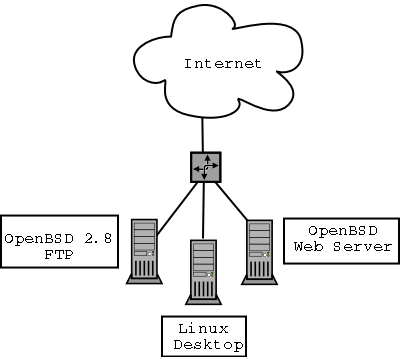
\includegraphics[width=0.5\linewidth]{images/home_network.png}
		\caption{figure \cite{example}}
		\label{broker}
	\end{center}
\end{figure}

